\chapter*{Introdução}
\label{ch:introduction}

\begin{chapquote}{Lewis Carroll, \textit{Alice in Wonderland}}
\enquote{Mas eu não quero me encontrar com gente louca}, observou Alice. \enquote{Oh, você não pode evitar isso}, replicou o Gato: \enquote{todos nós aqui somos loucos. Eu sou louco,você é louca}. \enquote{Como você sabe que eu sou louca?}, disse Alice. \enquote{Deve ser}, disse o Gato, \enquote{Ou não estaria aqui.}
\end{chapquote}

Em outubro de 2018, Arjun Balaji fez uma pergunta inofensiva, \textit {O que você aprendeu com o Bitcoin?} Depois de tentar responder a essa pergunta em um tweet e falhar miseravelmente, percebi que as coisas que aprendi são numerosas demais para serem respondidas rapidamente.

As coisas que aprendi são, obviamente, sobre o Bitcoin - ou pelo menos relacionadas a ele. No entanto, enquanto alguns dos funcionamentos internos do Bitcoin são explicados, as próximas lições não são uma explicação de como o Bitcoin funciona ou o que é. Elas podem, no entanto, ajudar a explorar algumas das coisas que o Bitcoin toca: questões filosóficas, realidades econômicas, e inovações tecnológicas.

\begin{center}
  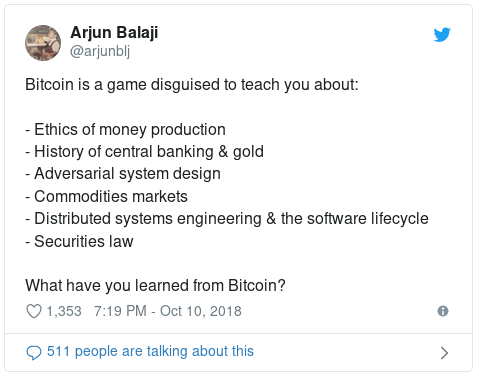
\includegraphics[width=7cm]{assets/images/the-tweet.png}
\end{center}

As \textit {21 Lições} são estruturadas em pacotes com sete lições cada, resultando em três capítulos. Cada capítulo examina o Bitcoin através de uma perspectiva diferente, extraindo as lições que podem ser aprendidas ao inspecionar essa estranha rede usando ângulos diferentes.

\paragraph{O \hyperref[ch: philosophy]{Capítulo 1}}{explora os ensinamentos filosóficos do Bitcoin. A interação de imutabilidade e da mudança, o conceito de verdadeira escassez, a concepção imaculada do Bitcoin, o problema da identidade, a contradição de replicação e da localidade, o poder da liberdade de expressão e os limites do conhecimento. }

\paragraph{O \hyperref[ch:economics]{Capítulo 2}}{explora os ensinamentos econômicos do Bitcoin. Lições sobre ignorância financeira, inflação, valor, dinheiro e sua história, o banco de reservas fracionárias e como o Bitcoin está reintroduzindo o dinheiro forte de uma forma astuta e indireta.}

\paragraph{O \hyperref[ch:technology]{Capítulo 3}}{explora algumas das lições aprendidas examinando a tecnologia do Bitcoin. Por que há força nos números, os reflexos sobre a confiança, por que dizer que o tempo dá trabalho, como o desenvolvimento lento mantendo tudo funcionando é um excelente recurso e não um bug, o que a criação do Bitcoin pode nos dizer sobre privacidade, por que os cypherpunks escrevem código (e não leis) e quais metáforas podem ser úteis para explorar o futuro do Bitcoin.}

~

Cada lição contém várias citações e links ao longo do texto. Se valer a pena explorar uma ideia com mais detalhes, você pode seguir os links que irão te levar para trabalhos relacionados nas notas de rodapé ou na bibliografia.

Embora algum conhecimento prévio sobre o Bitcoin seja benéfico para o entendimento, espero que essas lições possam ser digeridas por qualquer leitor curioso. Embora algumas das lições se relacionem entre si, cada uma deve ser capaz de ficar isolada por conta própria e pode ser lida de forma independente. Fiz o meu melhor para fugir do jargão técnico, embora algum vocabulário específico deste domínio seja inevitável.

Espero que minha escrita sirva de inspiração para que outros olhem abaixo da superfície e examinem algumas das questões mais profundas que o Bitcoin traz. Minha própria inspiração veio de uma infinidade de autores e criadores de conteúdo, a todos os quais sou eternamente grato.

Por último, mas não menos importante: meu objetivo ao escrever este livro não é convencê-lo de nada. Meu objetivo é fazer você pensar e te mostrar que o Bitcoin é muito mais do que aparenta ser. Eu nem posso te dizer o que é o Bitcoin ou o que o Bitcoin vai te ensinar. Você terá que descobrir por si mesmo.

\begin{quotation}\begin{samepage}
\enquote{Depois disto, não haverá retorno. Se tomar a pílula azul --- fim da história, vai acordar na sua cama e acreditar no que você quiser.  Se tomar a pílula vermelha \footnote{a pílula \textit{laranja}} --- você fica no País das Maravilhas, e eu vou mostrar até onde vai a toca do coelho.}
\begin{flushright} -- Morpheus
\end{flushright}\end{samepage}\end{quotation}

\begin{figure}
  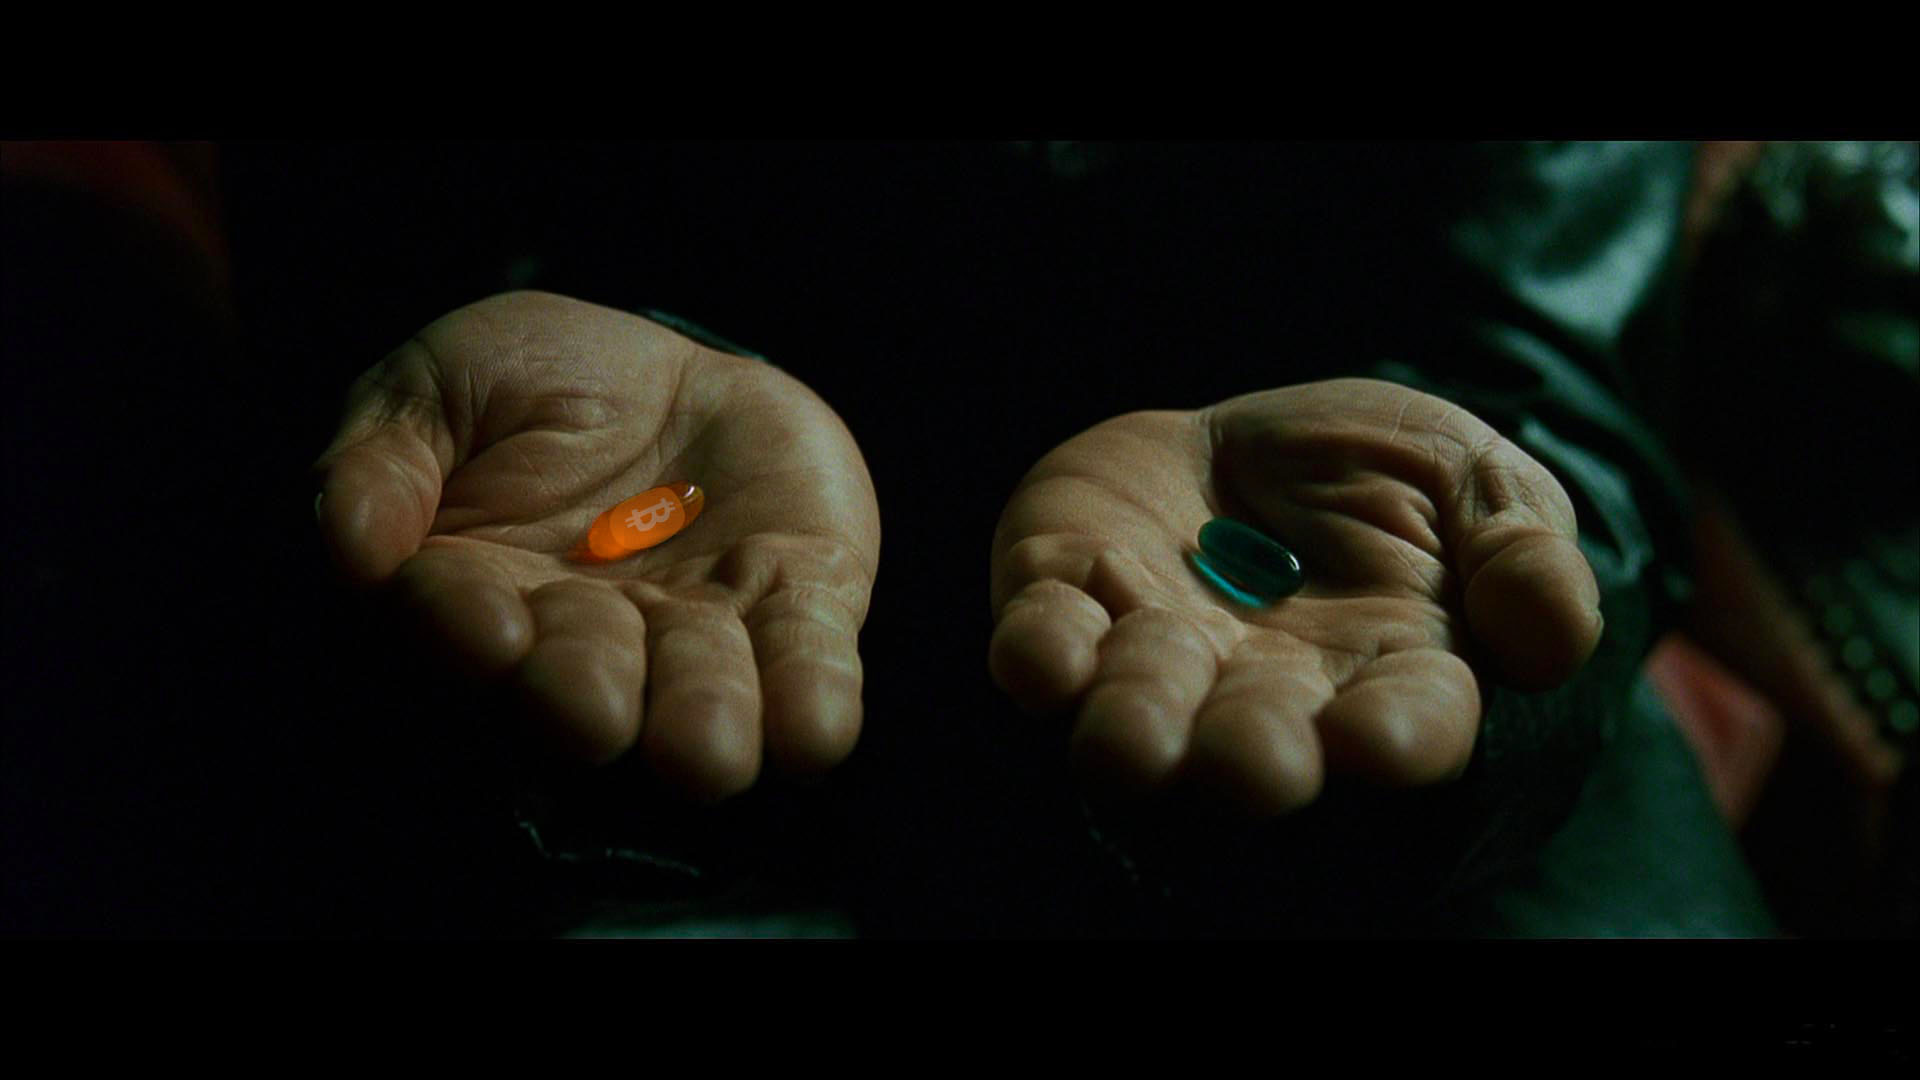
\includegraphics{assets/images/bitcoin-orange-pill.jpg}
  \caption*{Remember: All I'm offering is the truth. Nothing more.}
  \label{fig:bitcoin-orange-pill}
\end{figure}

%
% [Morpheus]: https://en.wikipedia.org/wiki/Red_pill_and_blue_pill#The_Matrix_(1999)
% [this question]: https://twitter.com/arjunblj/status/1050073234719293440
%
% <!-- Internal -->
% [chapter1]: {{ 'bitcoin/lessons/ch1-00-philosophy' | absolute_url }}
% [chapter2]: {{ 'bitcoin/lessons/ch2-00-economics' | absolute_url }}
% [chapter3]: {{ 'bitcoin/lessons/ch3-00-technology' | absolute_url }}
%
% <!-- Wikipedia -->
% [alice]: https://en.wikipedia.org/wiki/Alice%27s_Adventures_in_Wonderland
% [carroll]: https://en.wikipedia.org/wiki/Lewis_Carroll
